\documentclass[12pt,a4paper]{amsart}
\usepackage[UTF8]{ctex}
\usepackage{preamble}


\title{示波器的原理和使用及声速测量——实验报告}

\begin{document}

\maketitle

\section{基本信息}

\begin{enumerate}
  \item 班级:致理-数 02
  \item 姓名:谢泽钰
  \item 学号:2020012544
  \item 实验日期:2024 年 4 月 8 日
  \item 实验台号:20
\end{enumerate}


\section{实验仪器}

\subsection{Tektronix TBS1102B-EDU数字示波器}

Tektronix TBS1102B-EDU 数字示波器是一种双通道示波器,其带宽为 100MHz,采样率为 1GS/s,采用 7 英寸的液晶显示屏,可以显示两个波形,支持自动测量、触发、存储等功能。

\subsection{函数信号发生器}

Tektronix AFG1062 型函数信号发生器是一种多功能信号发生器,可以输出正弦波、方波、三角波等,其频率连续可调,范围可达 60MHz 高阻模式输出时信号峰峰值连续可调,最大可达 $20V$。

\section{实验原理}

\subsection{示波器显示波形原理}

要能够显示波形,必须同时在水平偏转板上加一扫描电压,使电子束光斑沿水平方向拉开。这种扫描电压的特点是电压随时间线性增加到最大值,然后快速降低至最小值,此后再重复这一过程。这种扫描电压随时间变化的关系曲线形同 “锯齿 故称 “锯齿波电压。当只有锯齿波电压加在水平偏转板上时,如果频率足够高,则荧光屏上只显
示一条水平亮线。\\

如果在竖直偏转板上(简称 $Y$ 轴)加正弦电压,同时在水平偏转板上(简称 $X$ 轴)加锯齿波电压,电子受竖直、水平两个方向的电场力的作用,电子的运动是两个相互垂直的运动的合成。当锯齿波电压与正弦电压的变化周期相等时,在荧光屏上将显示出完整周期的正弦电压波形。

\subsection{声速测量}

\subsubsection{空气中的声速}

在理想气体中,声波的传播速度为

\begin{equation}
    v = \sqrt{\frac{\gamma RT}{\mu}}
\end{equation}

式中 $\gamma = \frac{c_p}{c_V}$ 称为比热容比,即气体定压比热容与定容比热容的比值, $\mu$ 为气体的摩尔质量, $T$ 为绝对温度, $R=8.31441 J mol\cdot K$ 为普适气体常数。由(1)式可知,声速与温度成正比,与摩尔质量成反比。

\subsubsection{相位法测声速}

声波的传播速度与声波频率的关系为

\begin{equation}
    v = f\lambda
\end{equation}

只要测出声波的频率 $f$ 及波长 $\lambda$ ,便可求出声速 $v$。其中声波频率 $f$ 可通过测量声源的振动频率直接得到,波长 $\lambda$ 可以利用相位法来进行测量。波是振动状态的传播,也可以说是相位的传播。沿传播方向上的任何两点,如果其振动状态相同(同相)或者说其相位差为 $2\pi$ 的整数倍,这时两点间的距离应等于波长 $\lambda$ 的整数倍,即

\begin{equation}
    \lambda = n \vec{\lambda}\quad n = 1,2,3,\cdots
\end{equation}

\section{实验步骤}

\begin{enumerate}
    \item 连接电路
    \item 用示波器观察加在声波发射器上的电信号与超声波接收器输出的电信号
    \item 用相位法测波长
    \item 用声速公式计算声速
\end{enumerate}

\subsection{数据处理及结果}

\begin{table}[htbp]
    \centering
    \caption{自制信号源 4 种波形观测(被测信号输入到 CH1,交流耦合,衰减 X1)}
    \label{tab:score}
    \begin{tabular}{cccc}
    \toprule
    \textbf{波形} & \textbf{分度法} & \textbf{光标法} & \textbf{被测量值(以光标法为准)} \\
    \midrule
    正弦 & $V_{pp} = 2.76V$ & $V_{pp} = 2.76V$ & 电压有效值 $U_{eff} = 1.95V$ \\
    三角 & $T = 540 \mu s$ & $T = 540 \mu s$ & $T = 540 \mu s$ \\
    方波 & $V_{pp} = 4.30V$ & $V_{pp} = 4.32V$ & 1$V_{pp} = 4.32V$ \\
    脉冲 & $T = 530 \mu s$ & $T = 530 \mu s$ & $f = 1886.79 Hz$ \\
    \bottomrule
    \end{tabular}
    \end{table}

    \begin{table}[htbp]
        \centering
        \caption{驱动频率}
        \label{tab:score}
        \begin{tabular}{cccc}
        \toprule
        \textbf{变量} & \textbf{值} \\
        \midrule
        $f_1$ & $40.0003 kHz$ \\
        $f_2$ & $40.0003 kHz$ \\
        $f_3$ & $40.0005 kHz$ \\
        $f$ & $40.0004 kHz$ \\
        \bottomrule
        \end{tabular}
        \end{table}

        \begin{table}[htbp]
            \centering
            \caption{环境参数}
            \label{tab:score}
            \begin{tabular}{cccc}
            \toprule
            \textbf{测量时间} & \textbf{温度} & \textbf{相对湿度} \\
            \midrule
            实验前 & $25.6^{\circ}C$ & $29.9\%$ \\
            实验后 & $25.6^{\circ}C$ & $29.9\%$ \\
            \bottomrule
            \end{tabular}
            \end{table}

            \begin{table}[htbp]
                \centering
                \caption{声速实验数据}
                \label{tab:score}
                \begin{tabular}{cccc}
                \toprule
                \textbf{$i$} & \textbf{$x_i$/mm} \\
                \midrule
                1 & 0.0 \\
                2 & 8.99 \\
                3 & 17.93 \\
                4 & 26.86 \\
                5 & 35.03 \\
                6 & 43.83 \\
                7 & 53.06 \\
                8 & 61.59 \\
                9 & 70.52 \\
                10 & 79.01 \\
                11 & 86.93 \\
                \bottomrule
                \end{tabular}
                \end{table}

\subsection{理论声速计算}

\begin{equation}
    v = \sqrt{\frac{\gamma RT}{\mu}} = 331.5 \times \sqrt{1+\frac{25.16}{273.15}}\times\sqrt{1+0.31\times\frac{29.9\times 10^{-2}\times 0.03715 \times 10^5}{1.013\times 10^5}} = 347.1889 m/s
\end{equation}

\subsection{实验测量波长结果计算——直线拟合求波长}

\begin{figure}[htbp]
    \centering
    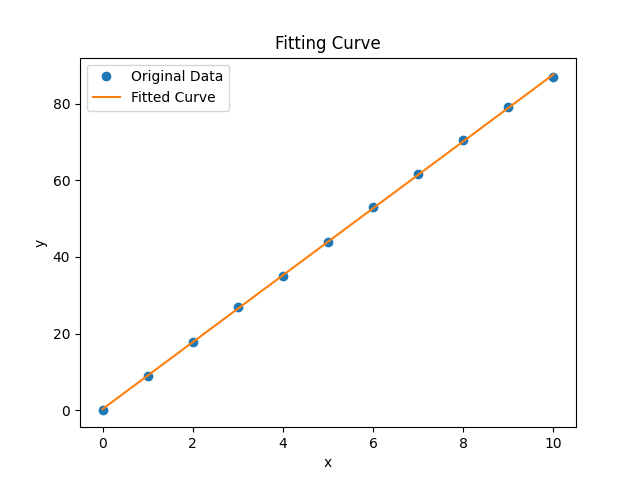
\includegraphics[width=0.8\textwidth]{plot.png}
    \caption{声速测量数据图}
\end{figure}

python 拟合结果

\begin{equation}
    x_i = 0.034136 + 8.727182 i
\end{equation}

因此波长

\begin{equation}
    \lambda = b = 8.727182 mm
\end{equation}

不确定度为 $2.909250$

\subsection{实验声速}

\begin{equation}
    \begin{aligned}
        &\lambda = 8.727182 \times 10^{-3} m\quad &T = f^{-1} = 2.5\times 10^{-5} s \\
        &v = \frac{\lambda}{T} = 349.087273 m/s   &\text{不确定度} \Delta v = 116.37 m/s
    \end{aligned}
\end{equation}

\section{相对偏差}

\begin{equation}
    \frac{|v_{\text{实验}} - v_{\text{理论}}|}{v_{\text{理论}}} = \frac{|349.087273 - 347.1889|}{347.1889} = 0.547\%
\end{equation}

\appendix

\bibliographystyle{unsrt}
{\footnotesize\bibliography{./library}}


\end{document}
